\documentclass[12pt]{article}
 
\usepackage[margin=1in]{geometry} 
\usepackage{amsmath,amsthm,amssymb}
\usepackage{graphicx}
 
\newenvironment{theorem}[2][Theorem]{\begin{trivlist}
\item[\hskip \labelsep {\bfseries #1:}]}{\end{trivlist}}

\begin{document}
 
% --------------------------------------------------------------
%                         Start here
% --------------------------------------------------------------
 
\title{A Curious Invariant Quantity in a Rectangle} % replace with an appropriate title, choose something shortish & descriptive
\author{Theron J Hitchman} % replace with your name, multiple authors go in alphabetical order by last name
 
\maketitle

{%
\centering
\textit{Communicated by: Ms. Prooffixer} % replace the name with the name of your referee(s)
\par
}
\hrule
\vspace{.2in}

We make a study of an interesting property of a rectangle: that the sum of the distances from a point on the rectangle to either diagonal is a constant. The basic idea of the proof is to find a way to make the quantity in question the length of a single unbroken segment, rather than as a sum.

This proof will rely on Conjecture 3.2, so I will hope someone proves that soon!
 
\begin{theorem}
Assume that conjecture 3.2 is a theorem, and hence each pair of opposite sides in a rectangle are congruent segments.

Let ABCD be a rectangle, and let P be a point lying on one of the sides. Let X and Y be the feet
of the perpendiculars from P to the diagonals BD and AC, respectively. Then the two segments PX and PY taken together are a constant. 

That is, if P and P' are any two such points, and X, Y, and X', Y' are the respective feet of the perpendiculars to the diagonals, then PX and PY taken together are the same as PX' and PY' taken together.
\end{theorem}
 
\begin{proof} We begin by choosing two points P and P' which lie on the segment CD. We shall make an argument for the theorem in this special case before moving to show that this special case is essentially enough for the whole result.

Let X,Y,X', and Y' be as in the statement of the theorem. Extend segment AD to a line, and then draw circle DA. Where these two objects meet, we find a new point E so that DA is congruent to DE. Then draw segment EC.

We claim that triangle DEC is congruent to triangle DAC. First, note that angle ADC is a right angle, by definition of a rectangle. Since the line DC cuts across the line AE at D, Euclid's Proposition I.13 shows that angle CDE is also a right angle. Therefore, segment AD is congruent to segment ED, angle ADC is congruent to angle EDC, and segment DC is congruent to itself. So by Euclid's Proposition I.8, the triangles ADC and EDC are congruent.


Okay. I gotta hold this example until we get some stuff proved about rectangles. Or I'll give away too much.

\begin{figure}[ht]
\centering
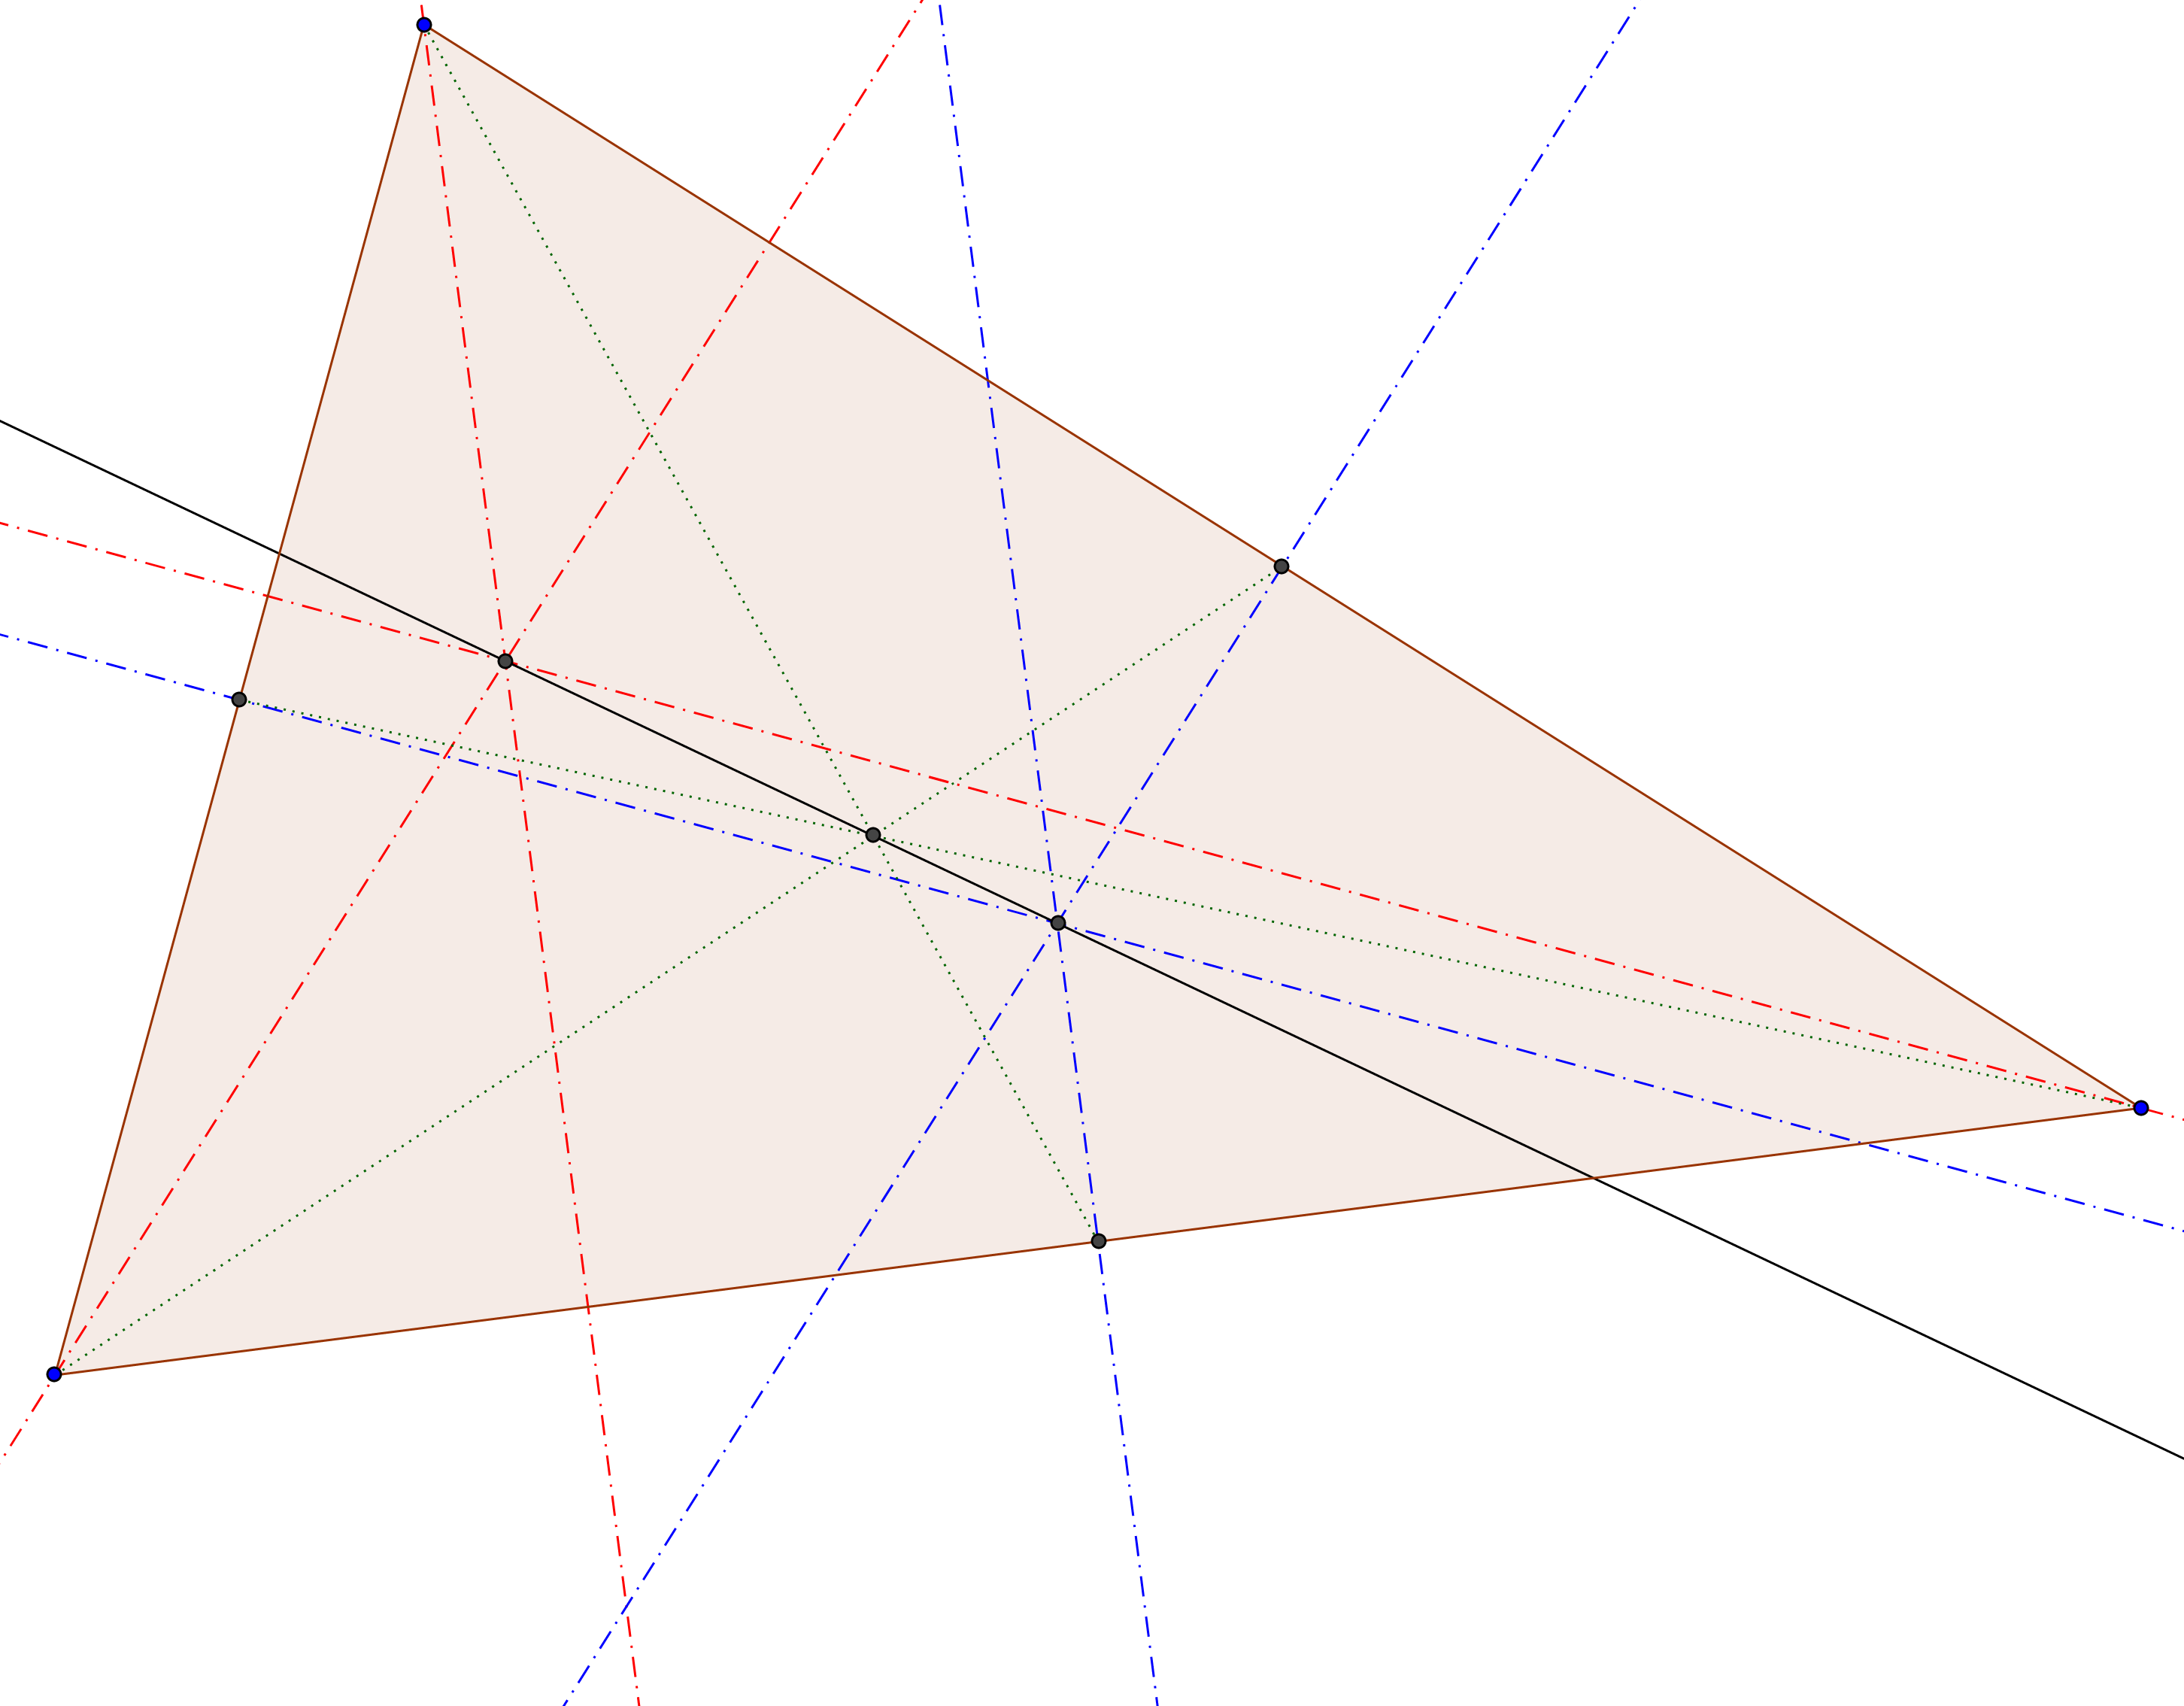
\includegraphics[width=.5\textwidth]{TEG_cover.png}
\caption{This is a picture of math.}
\end{figure}



\end{proof}
\end{document}